%!TEX TS-program = xelatex
%!TEX engine = xelatex

\documentclass{standalone}

\usepackage{fontspec}
\setmainfont{Fira Mono}
\usepackage{unicode-math}
\setmathfont[Scale=MatchUppercase]{STIX Two Math}
\setmathrm[Scale=MatchUppercase,
           BoldFont=STIX Two Text Bold]{STIX Two Math}
\setmathtt[Scale=MatchUppercase]{Fira Mono}
\usepackage{latexsym}

\usepackage{tikz}
\usetikzlibrary{arrows}

\begin{document}
  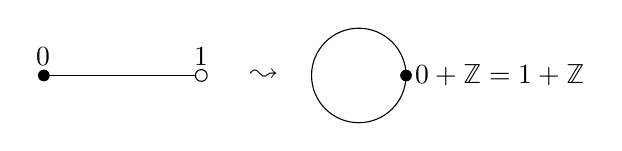
\begin{tikzpicture}
    \draw (0, 0) node[circle, fill, inner sep=1.5pt] {}
                 node[above] {$0$} --
          (2, 0) node[circle, draw, fill=white, inner sep=1.5pt] {}
                 node[above] {$1$};

    \node at (2.8, 0) {$\leadsto$};

    \begin{scope}[shift={(4, 0)}]
      \draw (0, 0) circle (0.6);
      \path (0.6, 0) node[circle,fill,inner sep=1.5pt] {}
            node[right] {$0 + ℤ = 1 + ℤ$};
    \end{scope}
  \end{tikzpicture}
\end{document}
